\documentclass[tikz,border=8pt]{standalone}
% Shared look for every TikZ diagram. Load with \input{../../tools/tikz-style.tex}
\usepackage[T1]{fontenc}
\usepackage{lmodern}
\renewcommand{\sfdefault}{lmr}  % diagrams use the same serif as the text
\usetikzlibrary{arrows.meta, positioning, shapes.geometric, calc, fit, backgrounds}
\definecolor{cblue}{HTML}{4C78A8}
\definecolor{corange}{HTML}{F58518}
\definecolor{cgreen}{HTML}{54A24B}
\definecolor{cred}{HTML}{E45756}
\definecolor{cpurple}{HTML}{B279A2}
\definecolor{cgrey}{HTML}{6B6B6B}
\tikzset{
  every picture/.style={font=\sffamily, line width=1.2pt},
  box/.style={draw=#1, fill=#1!12, rounded corners=4pt, align=center, inner sep=7pt, minimum height=1.1cm},
  box/.default=cgrey,
  arrow/.style={-{Stealth[length=3mm]}, draw=cgrey, line width=1.4pt},
  title/.style={font=\sffamily\bfseries\Large},
  note/.style={font=\sffamily\small, text=cgrey, align=center},
}
\AtBeginDocument{\hyphenpenalty=10000 \exhyphenpenalty=10000}

% One round of the particle filter: move every particle (motion model, own slip), weigh it by the reading
% (sensor model), resample in proportion to weight. The particle set carries the belief from round to round.
\begin{document}
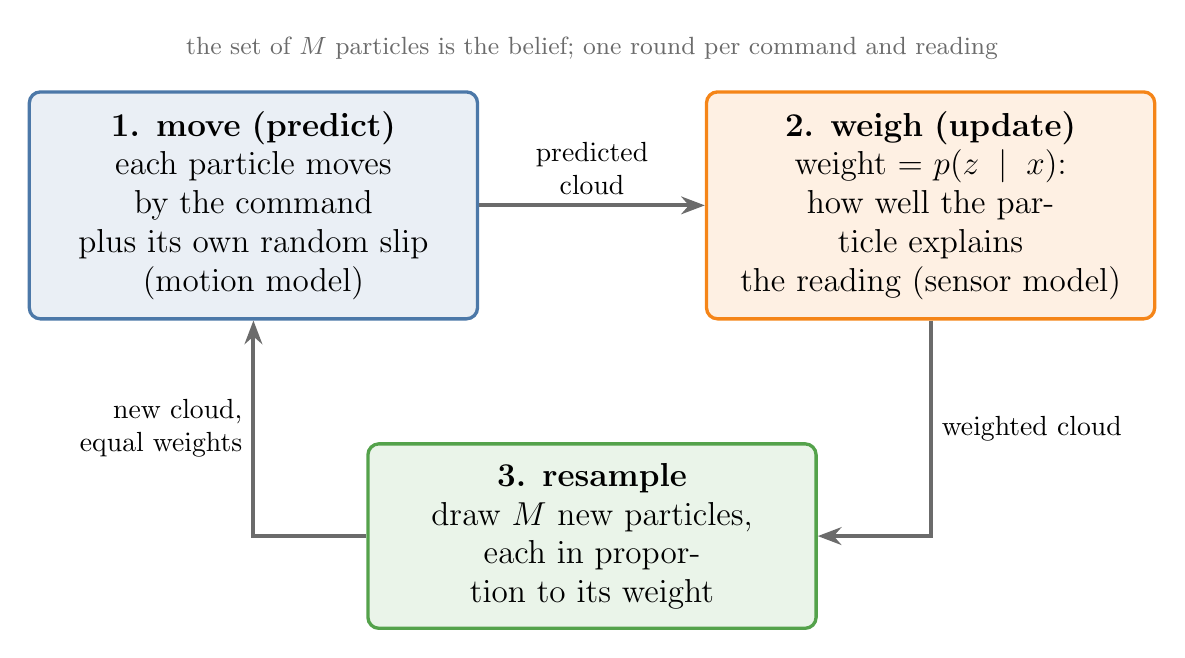
\begin{tikzpicture}[every node/.append style={font=\large}]
  \node[box=cblue, text width=5.2cm] (m) at (0,0) {\textbf{1. move (predict)}\\each particle moves by the command\\plus its own random slip\\(motion model)};
  \node[box=corange, text width=5.2cm] (w) at (8.6,0) {\textbf{2. weigh (update)}\\weight = $p(z \mid x)$:\\how well the particle explains\\the reading (sensor model)};
  \node[box=cgreen, text width=5.2cm] (r) at (4.3,-4.2) {\textbf{3. resample}\\draw $M$ new particles,\\each in proportion to its weight};
  \draw[arrow] (m) -- node[above, font=\normalsize, align=center] {predicted\\cloud} (w);
  \draw[arrow] (w.south) |- node[pos=0.25, right, font=\normalsize, align=left] {weighted cloud} (r.east);
  \draw[arrow] (r.west) -| node[pos=0.75, left, font=\normalsize, align=right] {new cloud,\\equal weights} (m.south);
  \node[note] at (4.3,2.0) {the set of $M$ particles is the belief; one round per command and reading};
\end{tikzpicture}
\end{document}
